\chapter{SLAM with Object Landmarks} \label{chap:object-slam}

In this chapter I present a SLAM formulation with object landmarks, which is scalable to medium sized indoor scenes and is robust to data association errors through the use of semantic information. Further I also present a compositional rendering method to render an accurate model frame at any given time during operation to propagate updated information to the front end in turn providing better initialization for the back end. This work is similar in spirit to a line of work started by \cite{salas-morenoSLAMSimultaneousLocalisation2013}. In this thesis however, the focus is on accurate trajectory estimation as well as object reconstruction. In essence, our work can be regarded as a bridge between feature based SLAM methods and dense SLAM methods.

\section{Related Literature}

In this section we review relevant literature in two aspects: classical geometry-based SLAM, and the application of deep semantic object detection in SLAM.
% Typically, SLAM methods incorporate semantics in two ways: (1) \textit{Loosely coupled}, where semantics are used post a completely independent map generation step. For instance, \cite{mccormac2017semanticfusion} generates a semantic map by fusing 2D segmentations in a post-processing step through bayesian updates, and \cite{grinvald2019volumetric} proposes a mapping scheme given camera trajectory to fuse geometric segmentation with Convolutional Neural Network (CNN) segmentations (2) \textit{Tightly coupled} where semantics are used directly to jointly optimize the map and camera trajectory. This tightly coupled treatment is called \textit{Object level SLAM}.

\subsection{Geometry-based SLAM}
\subsubsection{Problem formulation and pose optimization}
Modern geometry-based SLAM systems can be generally classified into \textit{feature-based} and \textit{direct} methods.
%
Feature-based SLAM systems ~\cite{mur-artalORBSLAM2OpenSourceSLAM2017, kleinParallelTrackingMapping2007} usually maintain a collection of sparse 3D \textit{point landmarks} corresponding to hand-crafted feature \textit{keypoints} detected in 2D images. In order to correct accumulated \textit{pose} error, \textit{i.e.,} drift, these methods resort to bundle adjustment \cite{triggsBundleAdjustmentModern2000} that jointly minimizes reprojection error between \textit{landmarks} and 2D \textit{keypoints} via \textit{pose} optimization. While being accurate in estimating trajectory, these approaches only come with sparse 3D maps that are less interpretable for visualization and recognition.
%
Direct SLAM~\cite{engelLSDSLAMLargeScaleDirect, engelDirectSparseOdometry2018} on the other hand, relies on pixel-wise projective data association between frames for odometry. Given relative poses between certain keyframes, pose graphs~\cite{dellaertFactorGraphsRobot2017} are formulated and optimized to obtain globally consistent poses without landmark constraints.

Our approach can be regarded as a bridge between the two approaches. We replace point landmarks with objects in feature-based SLAM. As a result, since pose constraints attached to objects can naturally replace reprojection error, we may directly convert such a landmark-pose constraint optimization to pose graph optimization (PGO).

\subsubsection{Map representation}
For \textit{dense} scene reconstruction, as introduced in Chapter \ref{chap:background} the volumetric Truncated Signed Distance Function (TSDF)~\cite{curlessVolumetricMethodBuilding1996} representation has been adopted and improved in several \textit{direct SLAM} frameworks. KinectFusion~\cite{newcombeKinectFusionRealtimeDense2011} introduced a plain $512^3$ grid for small scenes and objects. VoxelHashing~\cite{niessnerRealtime3DReconstruction2013} designed spatial hashing to scale this data structure to larger scenes. Similar implementations are available in CPU/GPU in the modern Open3D framework~\cite{zhouOpen3DModernLibrary2018, dongGPUAcceleratedRobust2019}, and we adopt this representation due to its ease of use.

\subsection{Object Instance Segmentation and Object based SLAM}
\subsubsection{Object instance segmentation}
In recent years, \textit{Region proposal} based Convolutional Neural Networks (R-CNN) \cite{renFasterRCNNRealTime2016} have established themselves as de-facto standards for object \textit{instance segmentation} from images. Amongst the literature, \textit{Mask-RCNN}~\cite{heMaskRCNN2018} and \textit{PointRend}~\cite{kirillovPointRendImageSegmentation2020} are the best off-the-shelf solutions.
In this work, we use \textit{PointRend} \cite{kirillovPointRendImageSegmentation2020}, which shows significant improvement over \cite{heMaskRCNN2018} by reformulating the mask generation as a rendering problem. In essence, this formulation is consistent with our tracking via compositional rendering module.

\subsubsection{Object based SLAM}
Applying aforementioned DNNs on 2D images, several works for RGBD and monocular SLAM have attempted to incorporate object instance detection. CubeSLAM~\cite{yangMonocularObjectPlane2019} and QuadricSLAM~\cite{nicholsonQuadricSLAMDualQuadrics2019} fit cuboids and quadrics, respectively, to detected objects to generate parameterized object landmarks. While improving the localization accuracy compared to baselines, these methods fail to densely map objects. \textit{MaskFusion}~\cite{runzMaskFusionRealTimeRecognition2018} adds labels to oriented point clouds and supports dense object visualization, but does not maintain persistent objects globally in a graph. \textit{Fusion++}~\cite{mccormacFusionVolumetricObjectLevel2018}, on the other hand, supports persistent dense reconstruction from fixed size $64^3$ voxel grids, yet is sensitive to voxel size tuning and may fail to adapt to objects at varying scales.
Our system utilizes scalable voxel grids that do not require much tuning to adjust to object scales. With a seamless CPU to GPU memory transfer implementation, larger environments can also be handled on-the-go.

% In this paper, we demonstrate an object graph formulation for simultaneous dense object reconstruction and accurate camera tracking, leveraging significant improvements in Deep Learning towards Object Detection and Object instance segmentation.


%and \citet{runz_maskfusion_2018} that propose object based representations for a scene. However, \cite{fusionPP} is based on unscalable discrete voxel grids, and uses lower resolution objects of $64^3$ to run feasibly, while \cite{runz_maskfusion_2018} is a surfel based method to track multiple objects and forgoes a factor-graph formulation and .
%More recently, \citet{xu2019mid}, proposes an octree datastructure, and utilizes a joint weighted photometric and geometric dense tracking similar to ours. This paper, however, focuses on tracking dynamic objects, and does not utilize a \textit{factor-graph} to jointly optimize camera, and \textit{correct} object poses.
% R-CNNs extract multiple region proposals, and individually classify and score the predictions to obtain labels and detection scores respectively. More recently, \citet{he2017mask} adds a parallel \textit{mask head} to generate object mask using Fully convolutional networks (FCN). Another line of work \cite{redmon2016you} predicts object bounding boxes directly by dividing an image into blocks and predicting probabilities.

% For directly segmenting \textit{3D data}, sparse convolution~\cite{4Dspatiotempro} and Key point convolution~\cite{kpconv} has started to gain attention in the community for its success on non-uniform point cloud data.

%In our work, we choose object detectors for images rather than point cloud, since we take RGBD data as raw input, and data association for objects from 2D is easier to obtain and update given depth maps and poses.

%\subsection{Object-based SLAM}
%\textbf{Sparse Feature based methods}. These approaches use object detection as opposed to object instance mask segmentation, to instantiate oriented 3D objects and fit cuboids \cite{yang2019cubeslam} or Quadrics \cite{quadric_slam}. They handle data association either by grouping detected keypoints into semantic labels, or assume known associations and define an Intersection-over-Union (IoU) overlap based error for optimization respectively. Although, these methods show improvement over baselines, they do not focus on object reconstruction fidelity. In contrast, our work uses a dense Hash-table based scalable volume data structure, which allows for accurate object reconstructions.

% \textbf{Direct dense methods}. SLAM++ %\cite{salas-moreno_slam_2013} was an early attempt towards SLAM with 3D object landmarks, that used a dense object representation. This method employed a dictionary of object descriptors generated through only geometric cues of each object model for data-association, and attempted camera trajectory optimization through multiple Frame to model ICP refinement between the live frame and \textit{each} detected object model. Further, a major limitation was that, it required pre-processed high quality mesh models of the expected objects in the scene prior to operation.

% The problem of high-fidelity 3D reconstruction has received substantial attention over the years. Key to high-quality 3D reconstruction is the choice of underlying representation for fusing sensor measurements of different modalities. Thus, most of the research on achieving globally consistent 3D models at scale uses the RGBD input that encapsulates the semantic as well as geometric (depth) information simultaneously. ~\citet{choi2015robust} proposes a framework that uses RGBD input to generate a very high-fidelity reconstruction of indoor scenes. They provide globally consistent models by optimizing across the entire pose trajectory. However, their approach requires offline processing and access to all the input frames resulting in hours of processing time, meaning real-time viability of refinement of reconstructed areas is almost impossible. Such joint global registration of multiple partially overlapping surfaces has also been considered by other works~\cite{huber2003fully,theiler2015globally}. To bridge this gap, this work proposes an object-centric pipeline for data association that reduce the expensive computational cost in registration.
% ~\citet{kinectfusion}'s seminal work KinectFusion introduced a new method and made RGBD reconstructions feasible. The key insight was to incorporate frame-to-model tracking as opposed to frame-to-frame tracking, which improved reconstruction accuracy significantly. Although it achieves impressive results, this approach still accumulates drift in the map estimate over long trajectories, since it does not retrospectively correct erroneous tracking. \citet{salas-moreno_slam_2013} extended KinectFusion and introduced an efficient pose graph formulation, that could be continually refined. However, this system required a detailed geometric model of the object a-priori. Further, ~\citet{fusionPP} propose an online object-level SLAM system wherein the 6DoF pose graph consists of only the reconstructed object instances. Using RGBD data of indoor scenes as their input, they leverage Mask-RCNN~\cite{Detectron2018} to generate 2D instance mask predictions of those objects. Consequently, these mask predictions are fused online into the per-object Truncated Signed Distance Function (TSDF) along with a 3D voxel mask to fuse the instance foreground. Although they demonstrate high quality object reconstruction within globally consistent loop-closed object SLAM maps, the memory usage scales cubically with the size of a TSDF. To combat the memory overflow, they propose integrating octree or voxel hashing into their pipeline to further boost run-time performance. Moreover, the system proposed by them is still susceptible to spurious detections resulting in a growing clutter of partial object reconstructions. As an improvement to this problem, they propose a learning-based mechanism for filtering and reconstructing objects.

\section{Compositional and Scalable Object SLAM} \label{sec: methodology}

 \subsection{System Overview}
Our pipeline can be divided into typical SLAM components and a deep perception module, connected by an object-based semantic map. Figure~\ref{fig:overview} provides an overview.

%
Our pipeline consists of 5 modules each running in a separate thread: semantic segmentation, frame-to-model odometry, object data association and map update, PGO, and compositional rendering.
%
Incoming RGBD frames are initially processed through  \textit{semantic segmentation} (\S\ref{subsec: segmentation})  to obtain instance masks, labels, and semantic descriptors, from DNNs for keyframes.
%
Then, odometry between the incoming live frame and the \textit{compositional render} from the map (\S\ref{subsec: rendering}) is estimated via \textit{frame-to-model odometry} (\S\ref{subsec: tracking}) to obtain relative poses.
%
Maintained objects visible in the frame are rendered given the estimated camera pose, and objects are associated with 2D instance detections to either integrate or initialize new objects in the global map (\S\ref{subsec: segmentation}).
%
Separately, a global factor-graph is updated to optimize the camera trajectory and object poses (\S\ref{subsec: optimization}). The optimized object poses are rendered to generate a compositional model of the scene for subsequent tracking (\S\ref{subsec: rendering}).

Before we discuss these modules in detail from \S\ref{subsec: tracking} to \S\ref{subsec: rendering}, we introduce core concepts and notations in \S\ref{subsec: notation}.

 \begin{figure}[htbp]
 	\centering
    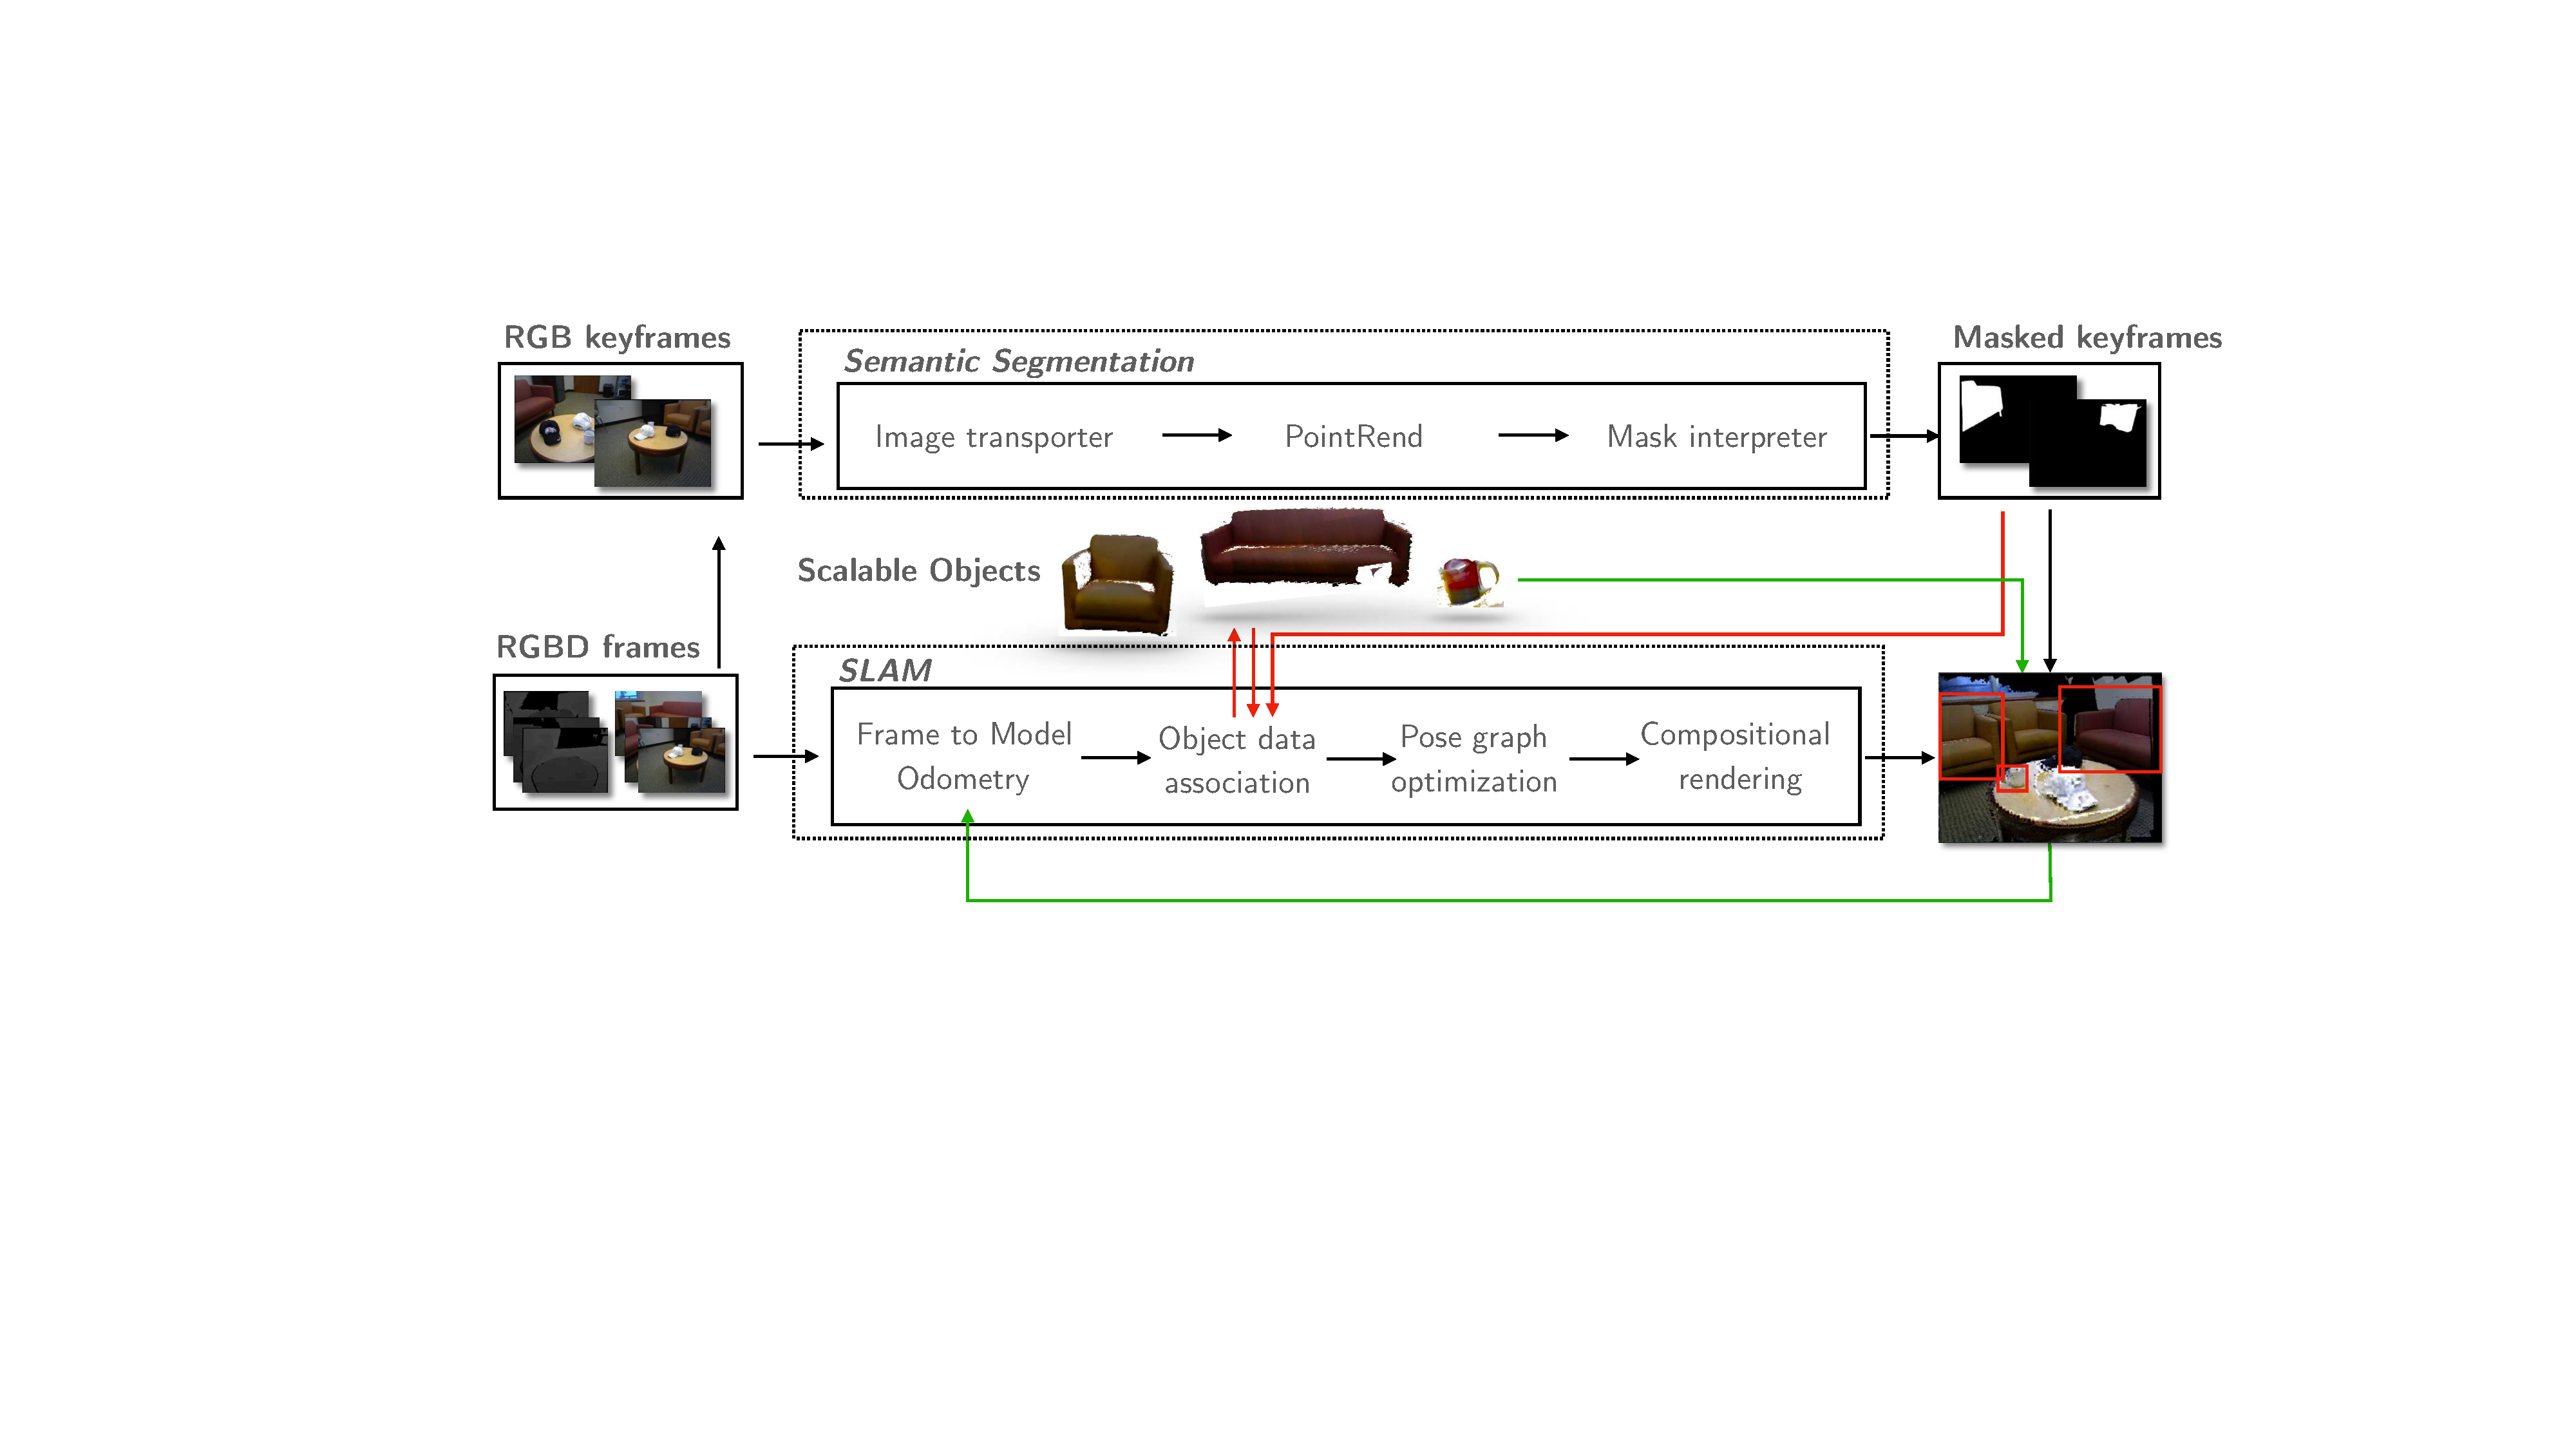
\includegraphics[width=\linewidth]{figs/icra2021-compressed.pdf}
    \caption{\label{fig:overview} System overview: Top shows the deep object segmentation pipeline that runs asynchronously, Masked keyframes from the segmentation pipeline are used in Data association and Map update (shown with red lines). Bottom shows the major stages of the reconstruction system, specifically object models are used in tracking via compositional raycasting (shown with green lines).}
 \end{figure}
\subsection{Core concepts and notations} \label{subsec: notation}
A background volume $V_B$ is a spatially-hashed voxel grid on GPU, where small $16^3$ subvolumes are allocated around observed 3D points. It is created and updated as a \textit{temporary} instance for stable tracking. An object volume $V_{O_i}$ is akin to the background volume, but persistently maintains the object label, ID, and corresponding object descriptors.

A 3D volume $V$'s properties, including surface vertex positions, normals, and colors can be mapped to 2D images given a camera pose $\mathbf{T} \in SE(3)$ and camera intrinsics defined as $K$ with ray-casting. We denote such \textit{rendered images} by \( \langle \mathcal{N}, \mathcal{V}, \mathcal{C} \rangle \)  for normal, vertex, and color maps respectively. They can be associated with input RGBD images $\langle \mathcal{I}, \mathcal{D}\rangle $ that consist of color ($\mathcal{I}$) and depth ($\mathcal{D}$) images via projective closest points.

We use subscripts and superscripts to indicate multiple coordinate frames used in our pipeline, including $C_i$ for $i$th camera, $O_j$ for $j$th object, and $W$ for background or world coordinate frame. For instance \(\langle \mathcal{N}_{C_s}, \mathcal{V}_{C_s}, \mathcal{C}_{C_s} \rangle \) represents 2D maps rendered from the volumes in the $C_s$ camera coordinate frame.
$\mathbf{T}_{O_j}^W \in SE(3)$ encodes a rigid transformation from object $j$ to world. Finally, we denote the respective measurements between nodes with variable $\mathbf{Z}$.

\subsection{Hybrid Frame to Model Odometry} \label{subsec: tracking}

In RGBD camera tracking, we seek to estimate the relative camera pose \(\mathbf{T}^{C_t}_{C_s}\) given an incoming RGBD target frame \( \langle \mathcal{I}_{C_t}, \mathcal{D}_{C_t}\rangle \) and a source model \( \langle \mathcal{N}_{C_{s}}, \mathcal{V}_{C_{s}}, \mathcal{C}_{C_{s}}\rangle \) of the scene rendered by placing a virtual camera at the previous camera frame ${C_s}$.

We accomplish this by minimizing the joint weighted dense geometric error residual $r_D$ and the photometric error residual $r_I$. The general energy function is formulated as in \cite{parkColoredPointCloud2017} by accumulating residual at every point $p \in \mathbb{Z}^2$ with a valid data association:
\begin{align}
    E(\mathbf{T}^{C_t}_{C_{s}}) = \sum_{p} (1 - \sigma) r_I^2(\mathbf{T}^{C_t}_{C_s}, p) + \sigma r_D^2(\mathbf{T}^{C_t}_{C_s}, p) \label{eq:1}
\end{align}
Here, we adapt the geometric ICP residual as the point-to-plane distance between the incoming depth map $\mathcal{D}$ and the rendered vertex and normal map $(\mathcal{V}_{C_s}, \mathcal{N}_{C_s})$ as follows, using the formulation in \cite{newcombeKinectFusionRealtimeDense2011}:
\begin{align}
    r_D(T^{C_t}_{C_s}, p) = \bigg(T^{C_t}_{C_{s}} \mathcal{V}_{C_s}( \hat{p} ) - \mathcal{V}_{C_{t}}(p )\bigg) \cdot \mathcal{N}_{C_{t}}( p ) \label{eq:2}
\end{align}
where $\mathcal{V}_{C_t}$ is the vertex map from unprojecting the input depth image $\mathcal{D}_{C_t}$.
Additionally, we use a photometric error residual to improve tracking robustness, which is defined as:
\begin{align}
    r_I(T^{C_t}_{C_s}, p) = \mathcal{C}_{C_s}(\hat{p}) - \mathcal{I}_{C_t}(p) \label{eq:3}
\end{align}
In equations (\ref{eq:2}) and (\ref{eq:3}), $\hat{p}$ is the correspondence of $p$ in the source frame, and is computed via \textit{warping}:
\begin{align}
    \hat{p} = K {\mathbf{T}^{C_t}_{C_s}}^{-1}\mathcal{D}_{C_t}(p)K^{-1}[p^\top, 1]^\top \label{eq:4}
\end{align}
It must be noted that the points $p$ are a subset of pixels with valid object-level data associations detailed in \S\ref{subsec: rendering}.

The energy function in equation \ref{eq:1} is minimized using the Gauss-Newton algorithm. We implement the minimization in a coarse to fine scheme using an image pyramid, on the GPU in parallel since each pixel acts independently in the energy function using \textit{reduction} with appropriate thread conflict handling as described in \cite{dongGPUAcceleratedRobust2019}.

\subsection{Object Instance Segmentation and Association} \label{subsec: segmentation}

\textbf{2D instance segmentation:} Object detection and instance masks are generated every $n^{th}$ frame (we choose $n=10$) in a separate thread from the \textit{PointRend} backend. \textit{PointRend} uses a Resnet-50-FPN backbone network to generate a convolutional feature map. In particular, after an empirical evaluation, we found that \textit{PointRend} provided better masks over \textit{Mask-RCNN}.

The semantic segmentation module maps incoming \textit{RGB} frame \(\mathcal{I}\) into a set of object labels $[l_1, \dots l_k]$, a set of binary object masks $M_n^i$ defined over $l \in \mathcal{L} \triangleq \{0, \dots, L_{max}-1\}$ object classes ($L_{max}=80$ in the MS-COCO dataset), bounding boxes $b \in \mathbb{N}^4$, and a probability distribution $p(l_i \mid \mathcal{I})$. We also extract the object feature map for the accepted object proposals, from the penultimate fully connected layer of the R-CNN from the object classifier head. We observe that these feature maps provide us with robust data association in ambiguous situations.
%
To obtain instance segmentation for frames not sent to the DNN, we warp the binary mask images from the most recent frame with a segmentation and fill the holes in the warped masks using the \textit{flood fill} algorithm.

Once the current camera pose and the semantic segmentation information are available, instance detections are associated with existing objects. Unmatched instance detections are used to initialize new object volumes.

\textbf{3D instance generation:} When an unmatched object is to be instantiated, the masked depth frame at $C_i$ is unprojected and transformed into the world frame to obtain the object point cloud:
\begin{align}
X_{W} = \mathbf{T}^W_{C_i} K^{-1} D_{C_i}(p) [p^\top, 1]^\top.
\end{align}
To obtain relatively high fidelity reconstruction, we adaptively calculate a conservative voxel length of
\begin{align}
    l = \gamma \| \max(X_W) - \min(X_W) \|_{\infty},
\end{align}
where $\min, \max$ operators are applied to all dimensions of $X \in \mathbb{R}^3$ simultaneously. We empirically use $\gamma = 1 / 64\sqrt{2}$, but due to the scalability of the volume our model is less sensitive to $\gamma$.
Finally, the object pose is simply chained by
\begin{align}
    \mathbf{T}_{O}^W = \mathbf{T}_{C_i}^{W} \bigg({\mathbf{T}_{C_i}^O}\bigg)^{-1},
\end{align}
where $\mathbf{T}_{C_i}^O = [I \mid t_{C_i}^O]$ with $t_{C_i}^O = \min(X_W) - t_{C_i}^W $. Each new object is also initialized with the object feature map from its corresponding instance mask.

\textbf{2D--3D semantic data association:}
To associate existing object volumes to 2D instances, visible objects are rendered (in \S\ref{subsec: rendering}) in the current frame. The rendered color map $\mathcal{C}$ is thresholded to obtain a virtual binary mask. An intersection over union (IoU) between the virtual binary mask $\hat{\mathcal{M}}$ and the instance masks $\mathcal{M}_i$ in the current frame is used as a scoring metric as defined in \cite{mccormacFusionVolumetricObjectLevel2018}.

As opposed to computing the $\argmax_{i}{\text{IoU}(\mathcal{M}_i, \hat{\mathcal{M})}}$, we associate objects as given below:
\begin{align}
    i = \argmin_{i \in \mathcal{S}} (\| f_i - \hat{f} \|_1),
\end{align}
where $\hat{f}$ and $f_i$ denote feature map of the object render (identical to the object in question), and the instance masks respectively and $\mathcal{S} \triangleq \{i : \text{IoU}(\mathcal{M}_i, \hat{M}) > 0.2\}$.
Associating object renders to instance masks in this manner prevents incorrectly fusing object instances between nearby similar objects, in cases where there is large accumulated drift.

% In practice, we reuse the object render generated after pose-graph optimization from the previous frame, for improved performance, as \textit{ray-casting} is the largest bottleneck on the system.

For subsequent fusion of a 2D instance detection to its associated 3D object, the instance mask---containing the object foreground---and the bounding box mask---containing both the foreground and background are used. Similar to \cite{mccormacFusionVolumetricObjectLevel2018} we integrate the object in both the foreground and background through a weighted average of TSDF, color, and additionally maintain binomial foreground-background count variables for each voxel. This smoothes out artifacts from integration of 2D instances with spurious masks (see illustration in Figure~\ref{fig:object-integration}).

\begin{figure}[htpb]
    \centering
    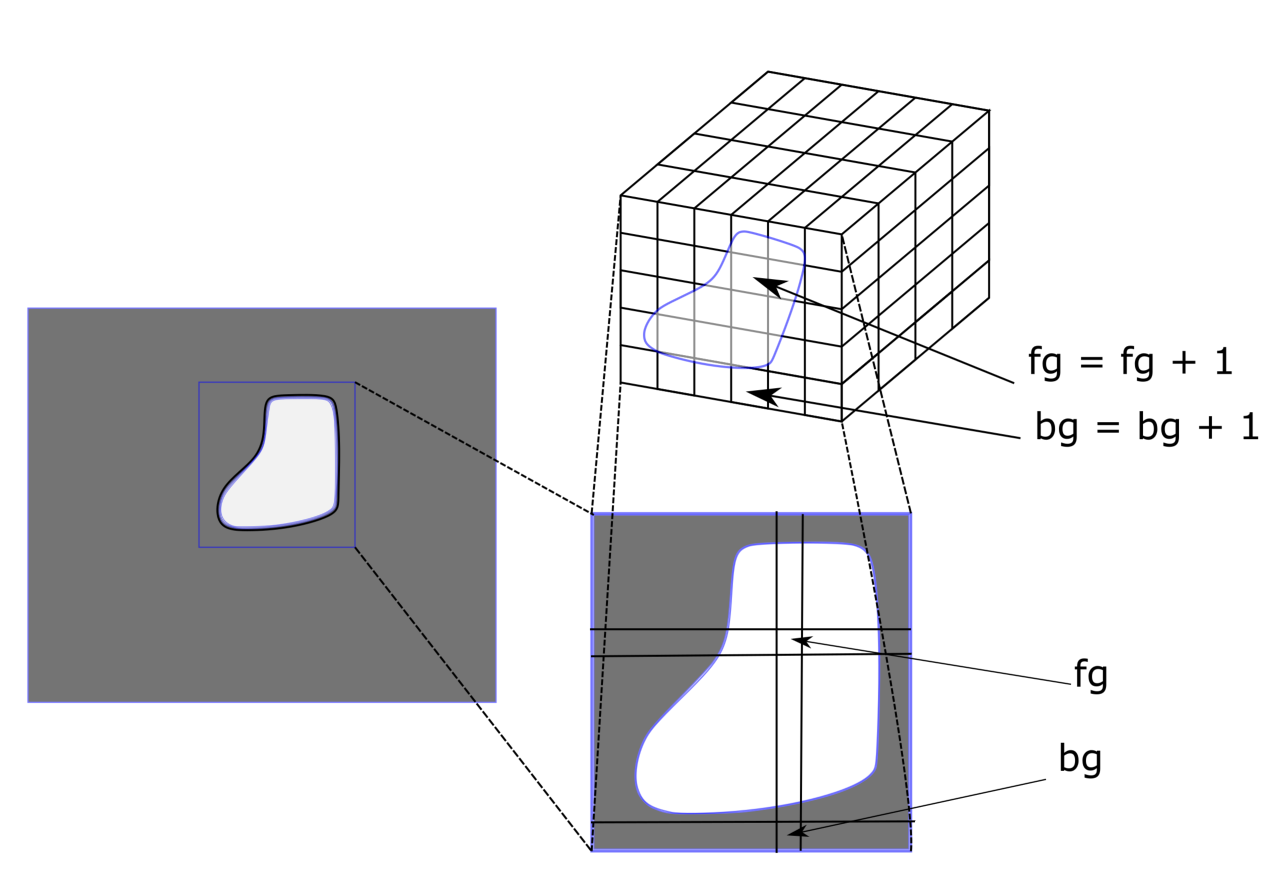
\includegraphics[width=0.8\linewidth]{figs/object-integration.png}
    \caption{Each pixel is a binomial trial given a latent foreground probability of the associated voxel. By maintaining foreground and background counts, we estimate the expected latent probability required during rendering.}%
    \label{fig:object-integration}
\end{figure}

Finally, we update the object feature map by a gated weight average:
\begin{align}
    f_t = \frac{w_{t-1} \cdot f_{t-1} + \mathcal{H}(f_{t-1}, f_{in}) \cdot f_{in}}{w_{t-1} + \mathcal{H}(f_{t-1}, f_{in})}\\
    \mathcal{H}(f_{t-1}, f_{in}) = \frac{\textrm{sgn}(\lambda - ||f_{t-1} - f_{in}||_1) + 1}{2}
\end{align}
where $\mathcal{H}$ is the Heaviside step function that hard-filters outlier input feature map $f_{in}$ compared to the maintained object feature map $f_{t-1}$ with weight $w_{t-1}$ controlled by the threshold $\lambda$.


\subsection{Factor Graph Optimization} \label{subsec: optimization}

As we have mentioned before, a background volume is maintained for stable tracking and to handle \textit{objectless} frames. The background volume additionally maintains the ratio ($r$) of visible volume units in the current camera frustum to the total number of allocated volume units in the volume. A low ratio implies that the camera may have moved away from a particular part of the scene. Pose graph optimization is conditionally triggered when the background volume is reset owing to low ratio of visible units ($r < 0.2$) and when there are new objects added into the graph.

Our object factor graph formulation is similar to \cite{salas-morenoSLAMSimultaneousLocalisation2013, mccormacFusionVolumetricObjectLevel2018}. The variable nodes $\mathcal{X} = \{\mathbf{x}_1, \dots \mathbf{x}_N\}$ are partitioned into camera pose variables $\mathbf{T}^{W}_{C_i} \in SE(3)$ and object pose variables $\mathbf{T}^W_{O_j} \in SE(3)$. The first camera pose is initialized as the world frame $W$.

Assuming a Gaussian noise model, the \textit{MAP} inference problem with the above variable nodes reduces to solving the following non-linear least squares optimization:
\begin{align}
    \mathcal{X}^* = \argmin_{\mathcal{X}} \Big( \sum_{k \in |C|} \|  \mathbf{Z}^{C_k}_{C_{k-1}} \ominus \mathbf{T}^{C_k}_{C_{k-1}} \|_{\Sigma_{k,k-1}}^2 + \sum_{j \in |\mathcal{O}|, k \in |\mathcal{C}|} \| \mathbf{Z}^{O_j}_{C_k} \ominus \mathbf{T}^{O_j}_{C_k} \|_{\Sigma_{o_j, k}}^2 \Big)
\end{align}
where the operator $ \mathcal{Y} \ominus \mathcal{X} = \text{Log}(\mathcal{X}^{-1} \mathcal{Y})$ expresses the relative error in the local tangent vector space \cite{solaMicroLieTheory2020}. $\Sigma_{k, k-1}$ denotes the covariance between relative camera pose measurements,  $\Sigma_{o_j, k}$ is the covariance in the camera to object measurement. They can be approximated by information matrices computed from \textit{odometry}, however, empirically we found that a constant information matrix can achieve reasonable results. We obtain the relative camera measurements $\mathbf{Z}^{C_k}_{C_{k-1}}$ from \textit{frame to model odometry} (\S\ref{subsec: tracking}), and obtain frame to object measurements $\mathbf{Z}^{O_j}_{C_k}$ by performing an additional Gauss Newton iteration with only the object pixels. Finally, the expected relative camera pose $\mathbf{T}^{C_k}_{C_{k-1}}$ and expected camera object pose $\mathbf{T}^{O_j}_{C_k}$ used in the factors are calculated as:
\begin{align}
    \mathbf{T}^{C_k}_{C_{k-1}} &= \bigg({\mathbf{T}^{W}_{C_k}}\bigg)^{-1} \mathbf{T}^{W}_{C_{k-1}}, \\
    \mathbf{T}^{O_j}_{C_k} &= \bigg({\mathbf{T}^{W}_{O_j}}\bigg)^{-1} \mathbf{T}^{W}_{C_k}.
\end{align}

We solve the optimization in GTSAM \cite{FactorGraphsGTSAM2019} using Levenberg Marquardt. Since the entire object volume is transformed as a rigid body, the object volumes remain unchanged in memory after optimization. We note that this circumvents the time-consuming re-integration that usually takes place in volumetric methods after PGO \cite{whelanElasticFusionDenseSLAM2015}.

\subsection{Compositional Rendering} \label{subsec: rendering}
Compositional rendering is a serialized operation that generates normal, vertex, and color maps by ray-casting 3D objects in the viewing frustum into 2D object instances, and is illustrated in Figure~\ref{fig:comp-render}.

\begin{figure}[htpb]
    \centering
    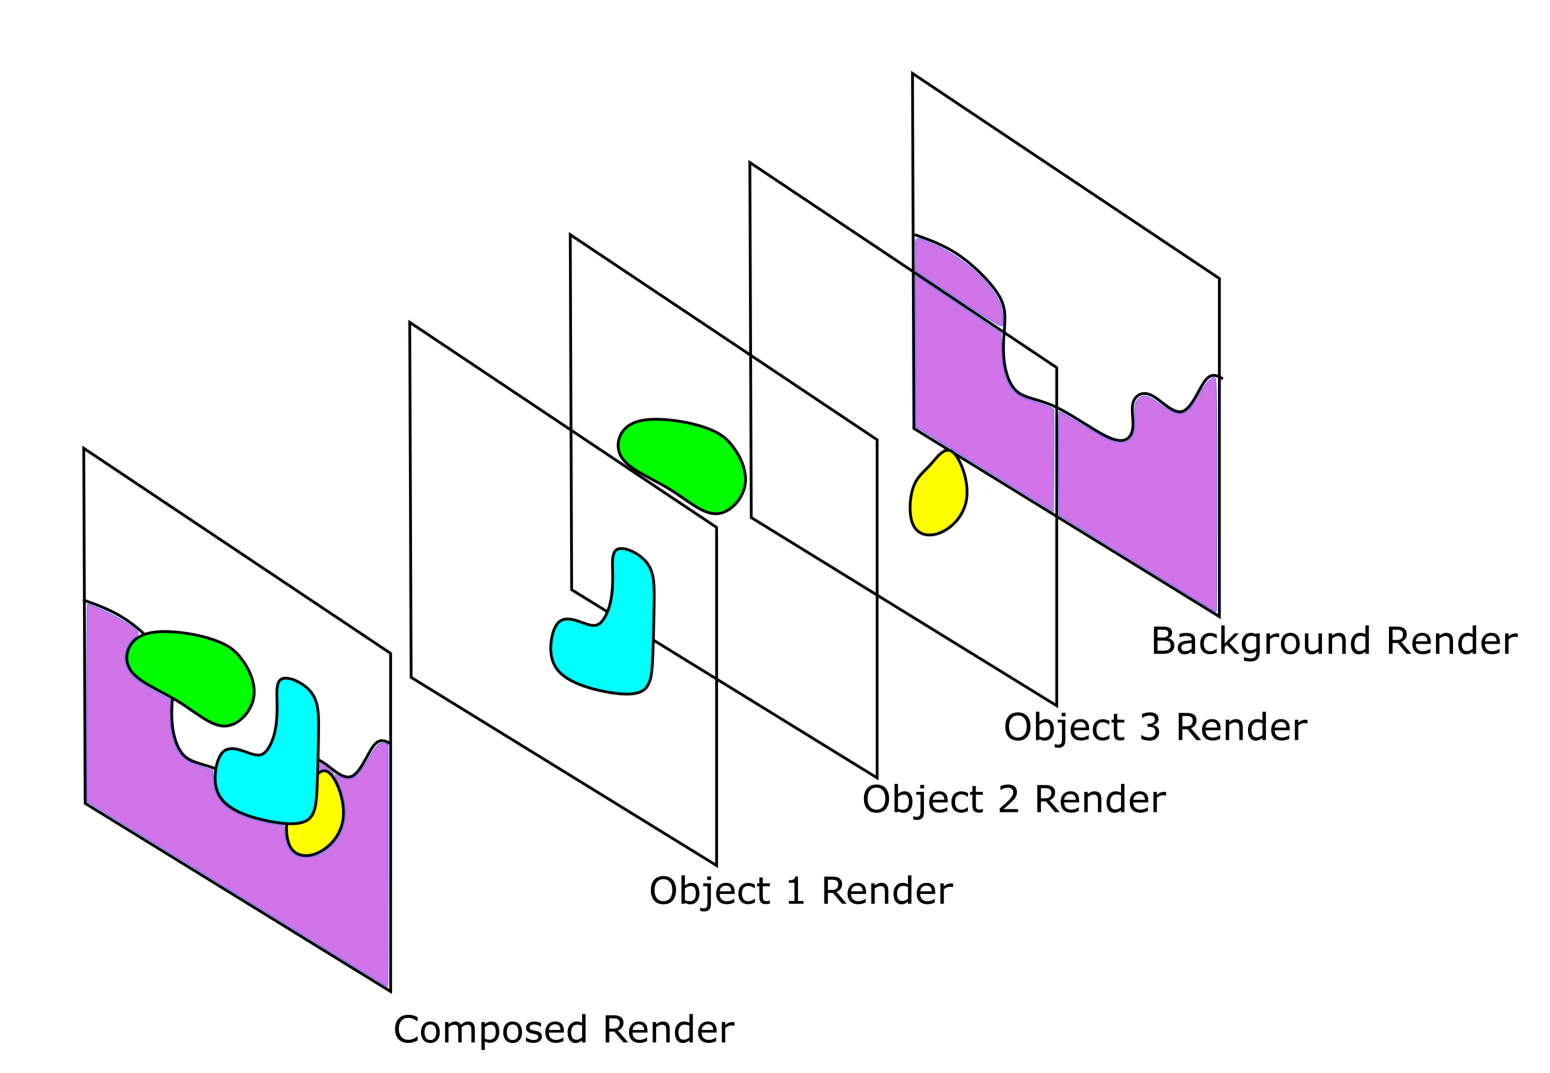
\includegraphics[width=0.8\linewidth]{figs/comp-render.png}
    \caption{An illustration of compositional rendering.}%
    \label{fig:comp-render}
\end{figure}

\(\langle \mathcal{N}_{C_i}, \mathcal{V}_{C_i}, \mathcal{C}_{C_i} \rangle \) is in fact an aggregation of separate renderings from object volumes \(\langle \mathcal{N}_{C_i}^{V_{{O}_j}}, \mathcal{V}_{C_i}^{V_{{O}_j}}, \mathcal{C}_{C_i}^{V_{\mathcal{O}_j}} \rangle \) and the background volume \(\langle \mathcal{N}_{C_i}^{V_{B}}, \mathcal{V}_{C_i}^{V_{B}}, \mathcal{C}_{C_i}^{V_{{B}}}  \rangle \), depending on the masks. In particular, we render the background volume, based on a background mask that is constructed from the union of existing virtual object masks in the current frame, and associated instance masks.

Then, the composed per-pixel map model render can be obtained as follows:
\begin{align}
    &\hat{k} = \argmin_k \mathcal{V}_k(p)[z], ~k \in \{O_1, \cdots, O_n, B\} \\
    &\langle \mathcal{N}^*(p), \mathcal{V}^*(p), \mathcal{C}^*(p) \rangle = \langle  \mathcal{N}_{\hat{k}}(p), \mathcal{V}_{\hat{k}}(p), \mathcal{C}_{\hat{k}}(p) \rangle,
\end{align}
where $\hat{k}$ is the volume index corresponding to the minimum distance to camera center for pixel $p$.

\begin{figure}[htpb]
    \centering
    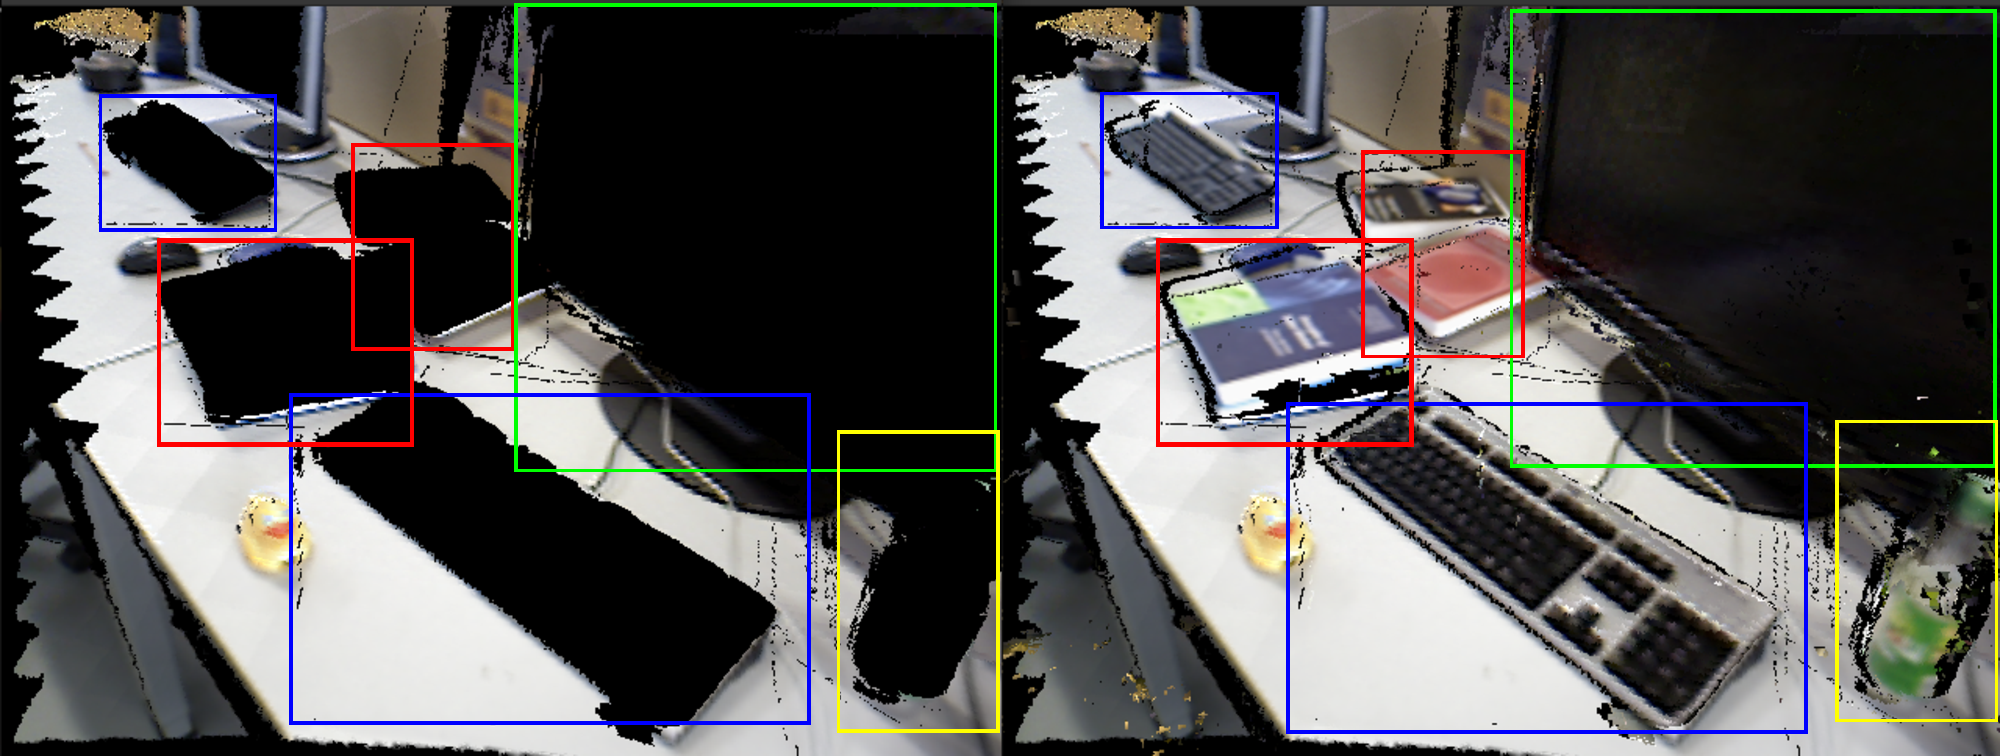
\includegraphics[width=\linewidth]{figs/compositional-render.pdf}
    \caption{Compositional rendering during reconstruction on TUM \textit{fr3\_long\_office\_household} dataset. Left shows the background render, and right shows the composed render. Compositionally rendered objects are shown in bounding boxes.}
    \label{fig:compositional_render}
\end{figure}

Object volumes not currently visible are downloaded from GPU into CPU memory. Note that downloading the object volume does not affect the optimization problem, since the object volumes are required only for integration and raycasting.
